%!TEX root = ../slides.tex
\section{Preliminary results}
\begin{frame}{Preliminary experimentation}{Materials and methods}
\small
\begin{block}{\small \textbf{Attributes evaluated}}
  \begin{itemize}
    \item Spatial-time accuracy.
    \item Energy consumption.
  \end{itemize}
\end{block}

\begin{block}{\small \textbf{Desktop version}}
  \begin{itemize}
    \item It features different modules of the proposed system (except from HAR module).
    \item It allows the quick evaluation of system performance through different parameter combinations.
    \item It includes a logic \emph{trajectory file} reader that simulates user motion.
  \end{itemize}
\end{block}

\begin{block}{\small \textbf{On-device trials}}
\begin{itemize}
  \item Two Nexus 6 smartphone units.% powered by Android 7 (Nougat) (Qualcomm Snapdragon 805 chipset, Adreno 420 GPU unit, a Quad-core 2.7 GHz mobile processor, 3GB in RAM).
  \item The smartphones were always carried together with the GPS logger device by a campus student.
  \item No mobile apps other than the developed middleware were executed by the smartphones.
  \item The smartphones were not employed for communication tasks (texting, calls).
\end{itemize}
\end{block}
\end{frame}

\begin{frame}{Preliminary experimentation}{Materials and methods}
\small 
\vspace{-0.5cm}
\begin{columns}
\begin{column}[T]{0.55\textwidth}
\begin{block}{\small \textbf{Ground-truth mobility information}}
  \begin{itemize}
    \item High frequency ($1~Hz$) location data collected employing a Qstarz BT-Q1000eX GPS logger.
    \item 6 trajectories collected by the same user, mostly using a vehicle as transportation mode.
  \end{itemize}
\end{block}
\end{column}

\begin{column}[T]{0.45\textwidth}
\begin{table}
\centering
\renewcommand{\arraystretch}{0.6}
\resizebox{0.83\textwidth}{!}{%
\begin{tabular}{@{}lll@{}}
\toprule
\multirow{2}{*}{\textbf{Stay Points Detector}} & \textbf{Time threshold} ($\delta_{time}$): & $45~min$ \\
\cmidrule[0.25pt]{2-3}
 & \textbf{Distance threshold} ($\delta_{distance}$): & $500~m$ \\

\cmidrule[0.25pt]{1-3}
\multirow{3}{*}{\textbf{Geofencing}} & \textbf{Radio distance} ($gf_{distance}$): & $250~m$ \\
\cmidrule[0.25pt]{2-3}
 & \textbf{Window size} ($gf_{ws}$): & 3 \\

\cmidrule[0.25pt]{1-3}
\textbf{Sampling period}: & \multicolumn{2}{l}{1 second} \\

\bottomrule
\end{tabular}%
}
\caption{Input parameters for the discovery of ground truth mobility information.}
\label{tab:exp-gt-input-parameters}
\end{table}
\end{column}
\end{columns}

\begin{table}
\centering
\renewcommand{\arraystretch}{0.8}
\resizebox{\textwidth}{!}{%
\begin{tabular}{@{}lrrrrrr@{}}
\toprule
\multicolumn{1}{c}{\textbf{Trajectory}} & 
\multicolumn{1}{c}{\textbf{Duration (days)}} & 
\multicolumn{1}{c}{\textbf{Inside SP time (minutes)}} &
\multicolumn{1}{c}{\textbf{In traj. time (minutes)}} &
\multicolumn{1}{c}{\textbf{Total SPs}} &
\multicolumn{1}{c}{\textbf{Total visits}} &
\multicolumn{1}{c}{\textbf{Individual SP weight}} \\
\midrule


% total minutes: 7 747.17
Trajectory 1 & 5.38 & 7,442.10 (96.06\%) & 305.07 (3.94\%) & 4 & 13 &
% 12 & 
\begin{tabular}[c]{@{}rr@{}}
Home: 72.25\% & Cinvestav: 26.03\%\\ 
Bob's place: 0.94\% & Store: 0.78\%\\
\end{tabular} \\

\cmidrule{1-7}
% total minutes: 8 714.15
Trajectory 2 & 6.05 & 8,348.42 (95.80\%) & 365.73 (4.20\%) & 6 & 21 & 
% 20 & 
\begin{tabular}[c]{@{}rr@{}}
Home: 69.67\% & Cinvestav: 26.51\%\\ 
Bob's place: 1.20\% & Park: 0.99\%\\ 
Store: 0.82\% & Stadium: 0.82\%\\
\end{tabular} \\

\cmidrule{1-7}
% total minutes: 8 849.57
Trajectory 3 & 6.15 & 8,542.12 (96.53\%) & 307.45 (3.47\%) & 6 & 31 & 
% 31 & 
\begin{tabular}[c]{@{}rr@{}}
Home: 67.94\% & Cinvestav: 24.50\%\\ 
Park: 2.94\% & Bob's place: 2.58\%\\ 
Fast food: 1.15\% & City center: 0.89\%\\
\end{tabular} \\

% total minutes: 10 396.62
\cmidrule{1-7}
Trajectory 4 & 7.22 & 10,024.63 (96.42\%) & 371.98 (3.58\%) & 2 & 16 & 
% 15 & 
\begin{tabular}[c]{@{}rr@{}}
Home: 66.50\% & Cinvestav: 33.50\%\\
\end{tabular} \\

\cmidrule{1-7}
% total minutes: 10 582.42
Trajectory 5 & 7.35 & 10,026.22 (94.74\%) & 556.20 (5.26\%) & 4 & 19 & 
% 18 & 
\begin{tabular}[c]{@{}rr@{}}
Home: 67.29\% & Cinvestav: 29.33\%\\ 
Cinema: 2.41\% & City center: 0.97\%
\end{tabular} \\

\cmidrule{1-7}
Trajectory 6 & 34.31 & 47,599.62 (96.34\%) & 1,807.52 (3.66\%) & 11 & 146 & 
% 145 & 
\begin{tabular}[c]{@{}rr@{}}
Home: 65.31\% & Cinvestav: 29.36\%\\ 
Home 2: 2.81\% & Fast food: 0.71\%\\
Bob's place: 0.37\% & Restaurant: 0.36\%\\ 
Store: 0.35\% & City center: 0.30\%\\
Workshop: 0.20\% & Store 2: 0.12\%\\
Workshop 2: 0.11\%\\
\end{tabular} \\ \bottomrule
\end{tabular}%
}
\caption{Mobility information of collected ground truth trajectories (SP=stay point).}
\label{tab:ground-truth-trajectories}
\end{table}
\end{frame}


% \subsection{Stay Points Detector spatial-time accuracy}
\begin{frame}{Preliminary experimentation}{\emph{Stay Points Detector} module spatial-time accuracy}
\small

\begin{columns}
\begin{column}[T]{0.55\textwidth}

\begin{block}{\small \textbf{Description}}
\begin{itemize}
  \item This experiment evaluates the spatial-time accuracy of the \emph{Stay Points Detector} module under different GPS sampling rates in terms of centroid distances and latencies.
\end{itemize}
\end{block}

\end{column}
\begin{column}[T]{0.45\textwidth}
\begin{table}
\centering
\renewcommand{\arraystretch}{0.6}
\resizebox{0.9\textwidth}{!}{%
\begin{tabular}{lll}
\toprule
\multirow{2}{*}{\textbf{Stay Points Detector}} & \textbf{Time threshold} ($\delta_{time}$): & $45~min$ \\
\cmidrule[0.25pt]{2-3}
 & \textbf{Distance threshold} ($\delta_{distance}$): & $500~m$ \\

\cmidrule[0.25pt]{1-3}
\textbf{Sampling periods}: & \multicolumn{2}{l}{30, 60, 90, 120, 150, 180 seconds.} \\

\cmidrule[0.25pt]{1-3}
\textbf{Trajectories}: & \multicolumn{2}{l}{All ground truth trajectories.} \\
\bottomrule
\end{tabular}
}
\caption{Input parameters for the spatial-time accuracy of stay points experiment.}
\label{tab:exp-1-input-parameters}
\end{table}
\end{column}
\end{columns}

\vspace{-0.5cm}
\begin{block}{\small \textbf{Results}}
\begin{columns}
\begin{column}{0.65\textwidth}
\begin{figure}
  \centering
  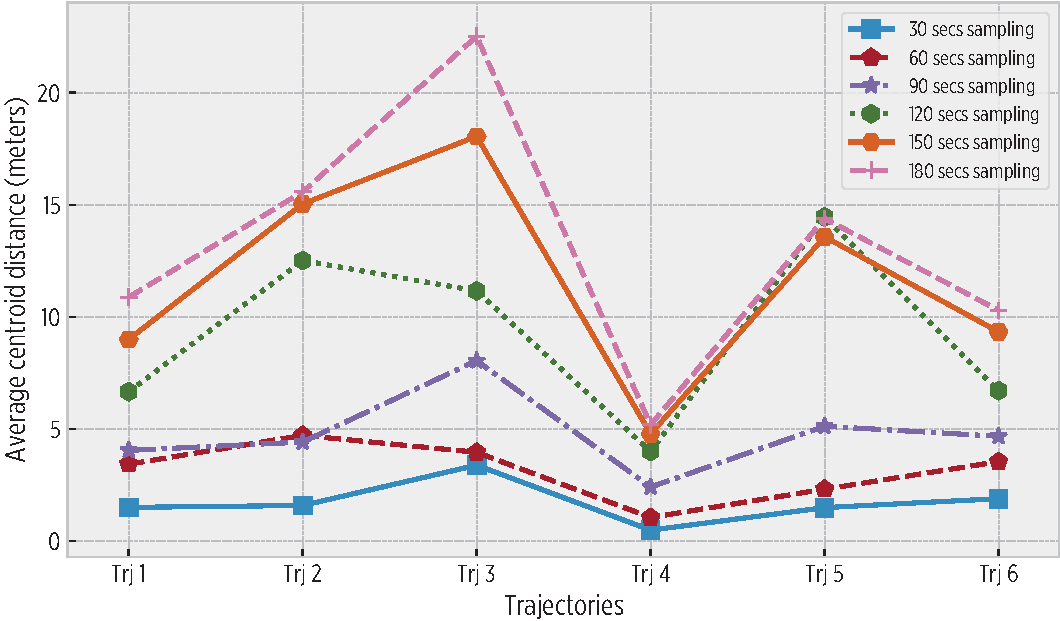
\includegraphics[width=0.99\textwidth]{vectors/experiments/exp-1/exp-1-centroid-distance}
\end{figure}
\end{column}
\begin{column}{0.3\textwidth}
\captionof{figure}{The impact of different sampling periods on the centroid distance of identified stay points in each trajectory. A maximum centroid distance of $22.52~m$ is identified when employing the 180 seconds sampling period.}
\end{column}
\end{columns}

\end{block}
\end{frame}

\begin{frame}{Preliminary experimentation}{\emph{Stay Points Detector} module spatial-time accuracy: Results}
\vspace{-0.5cm}
\begin{table}
\centering
\renewcommand{\arraystretch}{0.8}
\resizebox{0.72\textwidth}{!}{%
\begin{tabular}{@{}lrrrrrr@{}}
\toprule
\multicolumn{1}{c}{\textbf{Trajectory}} & 
\multicolumn{1}{c}{\textbf{\begin{tabular}[c]{@{}c@{}}Sampling period\\(seconds)\end{tabular}}} & 
\multicolumn{1}{c}{\textbf{\begin{tabular}[c]{@{}c@{}}Live stay\\ points identified\end{tabular}}} & 
\multicolumn{1}{c}{\textbf{\begin{tabular}[c]{@{}c@{}}Average centroid\\ distance (meters)\end{tabular}}} & 
% \multicolumn{1}{c}{\textbf{\begin{tabular}[c]{@{}c@{}}Average diameter\\ distance (meters)\end{tabular}}} & 
% \multicolumn{1}{c}{\textbf{\begin{tabular}[c]{@{}c@{}}Average ST\\ difference (seconds)\end{tabular}}} & 
\multicolumn{1}{c}{\textbf{\begin{tabular}[c]{@{}c@{}}Average arrival\\ latency (seconds)\end{tabular}}} & 
\multicolumn{1}{c}{\textbf{\begin{tabular}[c]{@{}c@{}}Average departure\\ latency(seconds)\end{tabular}}} \\ 
\midrule
\multirow{6}{*}{Trajectory 1} 
 & 30 & 12 of 12 & 1.50 &   2.67 & 24.92 \\
 & 60 & 12 of 12 & 3.43 &   \textcolor{red}{\textbf{\emph{-12.33}}} & 17.42 \\
 & 90 & 12 of 12 & 4.04 &   15.17 & 32.42 \\
 & 120 & 12 of 12 & 6.66 &  \textcolor{red}{\textbf{\emph{-7.33}}} & 52.42 \\
 & 150 & 12 of 12 & 9.00 &  25.17 & 79.92 \\
 & 180 & 12 of 12 & 10.88 & 22.67 & 77.42 \\
 \cmidrule(l){1-6}

\multirow{6}{*}{Trajectory 2} 
 & 30 & 16 of 16 & 1.59 & 7.38 & 13.62 \\
 & 60 & 16 of 16 & 4.72 & 20.50 & 34.25 \\
 & 90 & 16 of 16 & 4.42 & 37.38 & 26.75 \\
 & 120 & 16 of 16 & 12.51 & 16.75 & 83.00 \\
 & 150 & 16 of 16 & 15.04 & \textcolor{red}{\textbf{\emph{-0.12}}} & 96.12 \\
 & 180 & 16 of 16 & 15.58 & 65.50 & 71.75 \\
 \cmidrule(l){1-6}

\multirow{6}{*}{Trajectory 3} 
 & 30 & 19 of 19 & 3.39 &  2.26 & 12.16 \\
 & 60 & 19 of 19 & 3.96 &  11.74 & 12.16 \\
 & 90 & 19 of 19 & 8.05 &  40.16 & 29.53 \\
 & 120 & 19 of 19 & 11.16  & 37.00 & 56.37 \\
 & 150 & 19 of 19 & 18.06  & 48.05 & 59.53 \\
 & 180 & 19 of 19 & \textcolor{green}{\textbf{22.52}} & 87.53 & 81.63 \\
 \cmidrule(l){1-6}

\multirow{6}{*}{Trajectory 4} 
 & 30 & 13 of 13 & 0.49 &  16.15 & 2.46 \\
 & 60 & 13 of 13 & 1.05 &  41.54 & 34.77 \\
 & 90 & 13 of 13 & 2.41 &  32.31 & 55.54 \\
 & 120 & 13 of 13 & 4.00 & 32.31 & 71.69 \\
 & 150 & 13 of 13 & 4.78 & 41.54 & 50.92 \\
 & 180 & 13 of 13 & 5.19 & 73.85 & 62.46 \\
 \cmidrule(l){1-6}

\multirow{6}{*}{Trajectory 5} 
 & 30 & 18 of 18 & 1.49 & 0.17 & 13.61 \\
 & 60 & 18 of 18 & 2.31 & 13.50 & 21.94 \\
 & 90 & 18 of 18 & 5.12 & \textcolor{red}{\textbf{\emph{-3.17}}} & 23.61 \\
 & 120 & 18 of 18 & 14.46 & 10.17 & \textcolor{red}{\textbf{\emph{-44.72}}} \\
 & 150 & 18 of 18 & 13.58 & 30.17 & \textcolor{red}{\textbf{\emph{-39.72}}} \\
 & 180 & 18 of 18 & 14.39 & 26.83 & \textcolor{red}{\textbf{\emph{-71.39}}} \\
 \cmidrule(l){1-6}

\multirow{6}{*}{Trajectory 6} 
 & 30 & 75 of 75 & 1.89 & 2.89 & 6.89 \\
 & 60 & \textcolor{blue}{\textbf{76 of 75}} & 3.54 & 8.49 & 24.89 \\
 & 90 & \textcolor{blue}{\textbf{76 of 75}} & 4.67  & 7.29 & 59.69 \\
 & 120 & \textcolor{blue}{\textbf{76 of 75}} & 6.71 & 29.29 & 77.69 \\
 & 150 & 75 of 75 & 9.33 & 42.89 & 113.29 \\
 & 180 & \textcolor{blue}{\textbf{76 of 75}} & 10.29 & 51.69 & 108.89 \\
 \bottomrule 
\end{tabular}
}
\caption{Spatial-time differences in detected stay points per sampling period (ST=stay time). The negative values in the ST difference and the arrival and departure latencies are caused by the combined effect of user mobility and sparse sampling rate on the \emph{StreamedZhen} algorithm, which generates stay points in subtly different coordinates with different time information.}
\end{table}
\end{frame}


% \subsection{Geofencing accuracy}
\begin{frame}{Preliminary experiments}{\emph{Geofencing} module spatial-time accuracy: Description}
\small 
\begin{block}{\small \textbf{Description}}
\begin{itemize}
  \item This experiment evaluates the spatial-time accuracy of the visits information detected by the \emph{Geofencing} module under different GPS sampling rates, in terms of missed visits, and arrival and departure distance-latency.
\end{itemize}
\end{block}

\begin{table}
\centering
\renewcommand{\arraystretch}{0.8}
\resizebox{0.6\textwidth}{!}{%
\begin{tabular}{lll}
\toprule
\multirow{2}{*}{\textbf{Geofencing}} & \textbf{Radio distance} ($gf_{distance}$): & $250~m$ \\
\cmidrule[0.25pt]{2-3}
 & \textbf{Window size} ($gf_{ws}$): & 3, 5, 7 \\

\cmidrule[0.25pt]{1-3}
\textbf{Sampling periods}: & \multicolumn{2}{l}{30, 60, 90, 120, 150, 180 seconds.} \\

\cmidrule[0.25pt]{1-3}
\textbf{Trajectories}: & \multicolumn{2}{l}{All ground truth trajectories.} \\

\cmidrule[0.25pt]{1-3}
\textbf{STM} & \multicolumn{2}{l}{Preloaded with corresponding ground truth stay points.} \\
\bottomrule
\end{tabular}
}
\caption{Input parameters for the spatial-time accuracy of Geofencing module experiment.}
\label{tab:exp-2-input-parameters}
\end{table}
\end{frame}

\begin{frame}{Preliminary experiments}{\emph{Geofencing} module spatial-time accuracy: Results}
\vspace{-0.5cm}
\begin{figure}
  \centering
  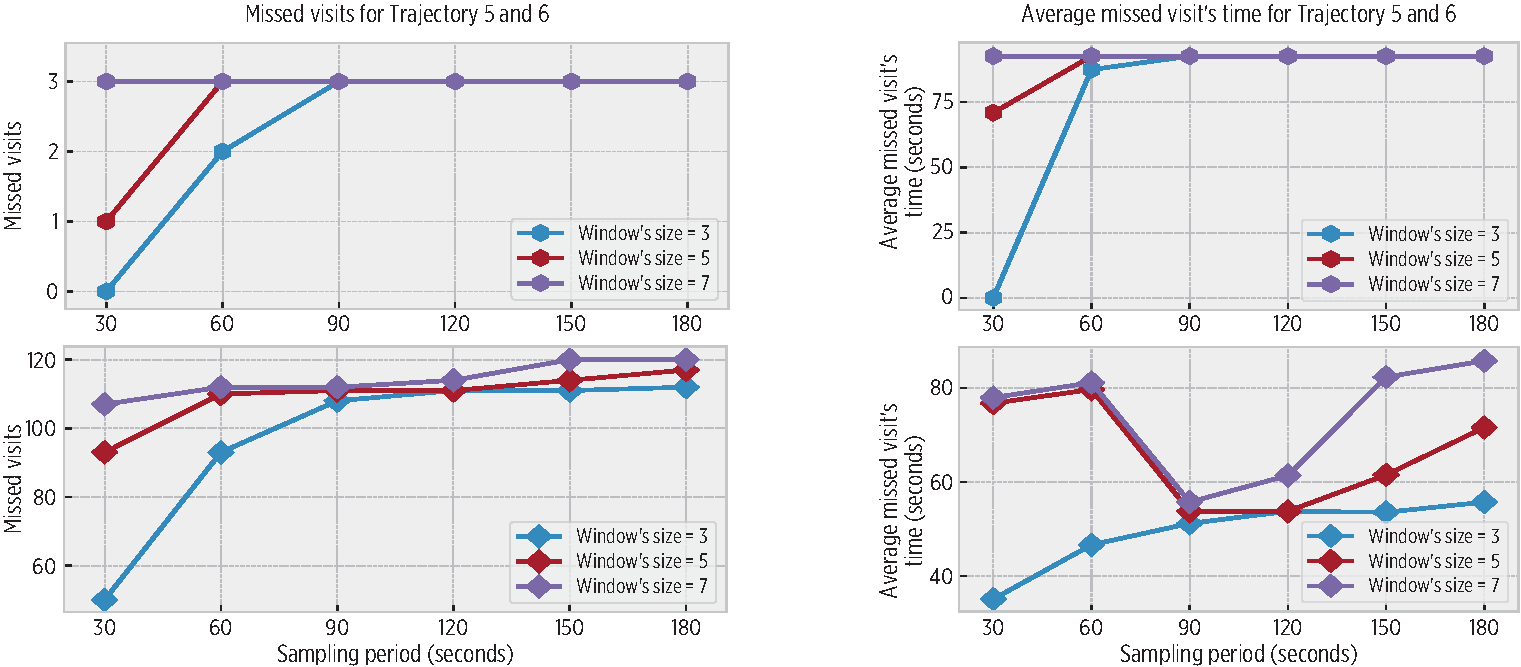
\includegraphics[width=0.78\textwidth]{vectors/experiments/exp-2/exp-2-visits-for-slides}
  \caption{Visits missed by the \emph{Geofencing} module for each combination of sampling period and window size values. The largest amount is obtained for the \emph{Trajectory 6}, given its length (more than 30 days). Nevertheless, they do not account for a considerable time in overall trajectories.}
\end{figure}
\end{frame}

\begin{frame}{Preliminary experiments}{\emph{Geofencing} module spatial-time accuracy: Results}
\vspace{-0.5cm}
\begin{figure}
  \centering
  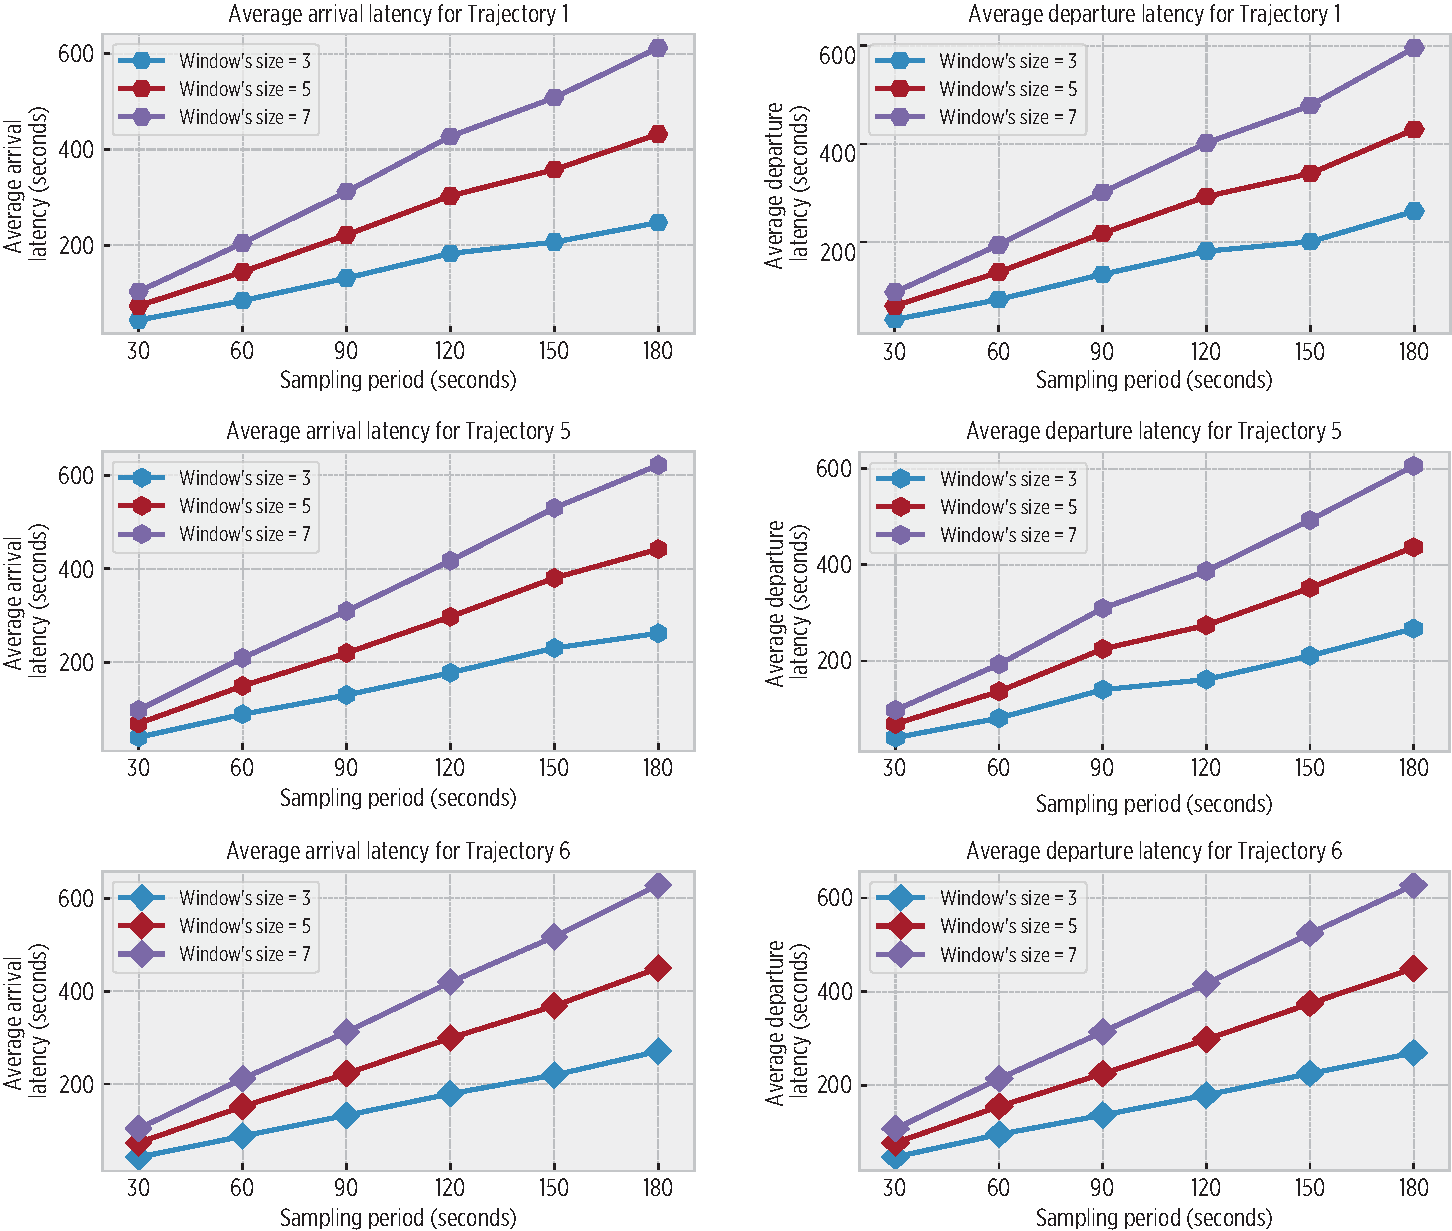
\includegraphics[width=0.75\textwidth]{vectors/experiments/exp-2/exp-2-latencies-for-slides}
  \caption{Arrival (left) and departure (right) latencies obtained by the Geofencing  module for each combination of sampling period and window length values. There is a tendency on the results as the shortest window’s sizes produce the shortest arrival latency values.}
\end{figure}
\end{frame}


% \subsection{Reaction to STM mobility mismatches}
\begin{frame}{Preliminary experiments}{Reaction to STM mobility mismatches: Description}
\begin{block}{\small \textbf{Description}}
{ 
\small
\begin{itemize}
  \item This experiment was focused on evaluating the ability of the system for reacting to mismatches in mobility information, with a particular emphasis on mismatch departure events.
  \item For some trials the information of the STM was intentionally modified by giving it longer stay times than those in the actual visits.
  \item The missed visits, the delay for detecting the temporal mismatches, and the departure latency were evaluated.
\end{itemize}
}
\end{block}

\begin{table}
\centering
\renewcommand{\arraystretch}{0.8}
\resizebox{0.75\textwidth}{!}{%
\begin{tabular}{@{}lll@{}}
\toprule

\multirow{3}{*}{\textbf{Geofencing}} & \textbf{Radio distance} ($gf_{distance}$): & $250~m$ \\
% \cmidrule[0.25pt]{2-3}
% & \textbf{Pivot parameter} ($gf_{pv}$): & center \\
 \cmidrule[0.25pt]{2-3}
 & \textbf{Window size} ($gf_{ws}$): & 3 \\

\cmidrule[0.25pt]{1-3}
\multirow{6}{*}{\textbf{Cognitive Controller}} & \multirow{2}{*}{\textbf{Sigmoid segments} ($\Theta_{domain\_segs}$):} & $(-5, -2.375), (-2.375, -1), (-1, 1), (1, 2.375), (2.375, 5)$ \\
 &  & $(-4, -2.375), (-2.375, -1), (-1, 1), (1, 2.375), (2.375, 5)$ \\
\cmidrule[0.25pt]{2-3}
 & \multirow{4}{*}{\textbf{Time separations} ($\Theta_{time\_sep}$):} & $[90, 150, 180, 150, 90]$ seconds \\
 &  & $[90, 120, 180, 120, 90]$ seconds \\
 &  & $[60, 150, 180, 150, 60]$ seconds \\
 &  & $[60, 120, 180, 120, 60]$ seconds \\

\cmidrule[0.25pt]{1-3}
\textbf{Trajectories} & \multicolumn{2}{l}{All ground truth trajectories.} \\

\cmidrule[0.25pt]{1-3}
\textbf{STM} & \multicolumn{2}{l}{\begin{tabular}[c]{@{}l@{}}Preloaded with ground truth stay points, with increased time (injured) in the proportions\\ $[5,10,15,\ldots,90,95,100]$ \%\end{tabular}}
%\begin{tabular}[c]{@{}l@{}}\\ \end{tabular}
\\
\bottomrule
\end{tabular}%
}
\caption{Input parameters for the reaction to mobility mismatches experiment.}
\label{tab:exp-3-input-parameters}
\end{table}
\end{frame}


\begin{frame}{Preliminary experiments}{Reaction to STM mobility mismatches: Results}
\begin{figure}
  \centering
  %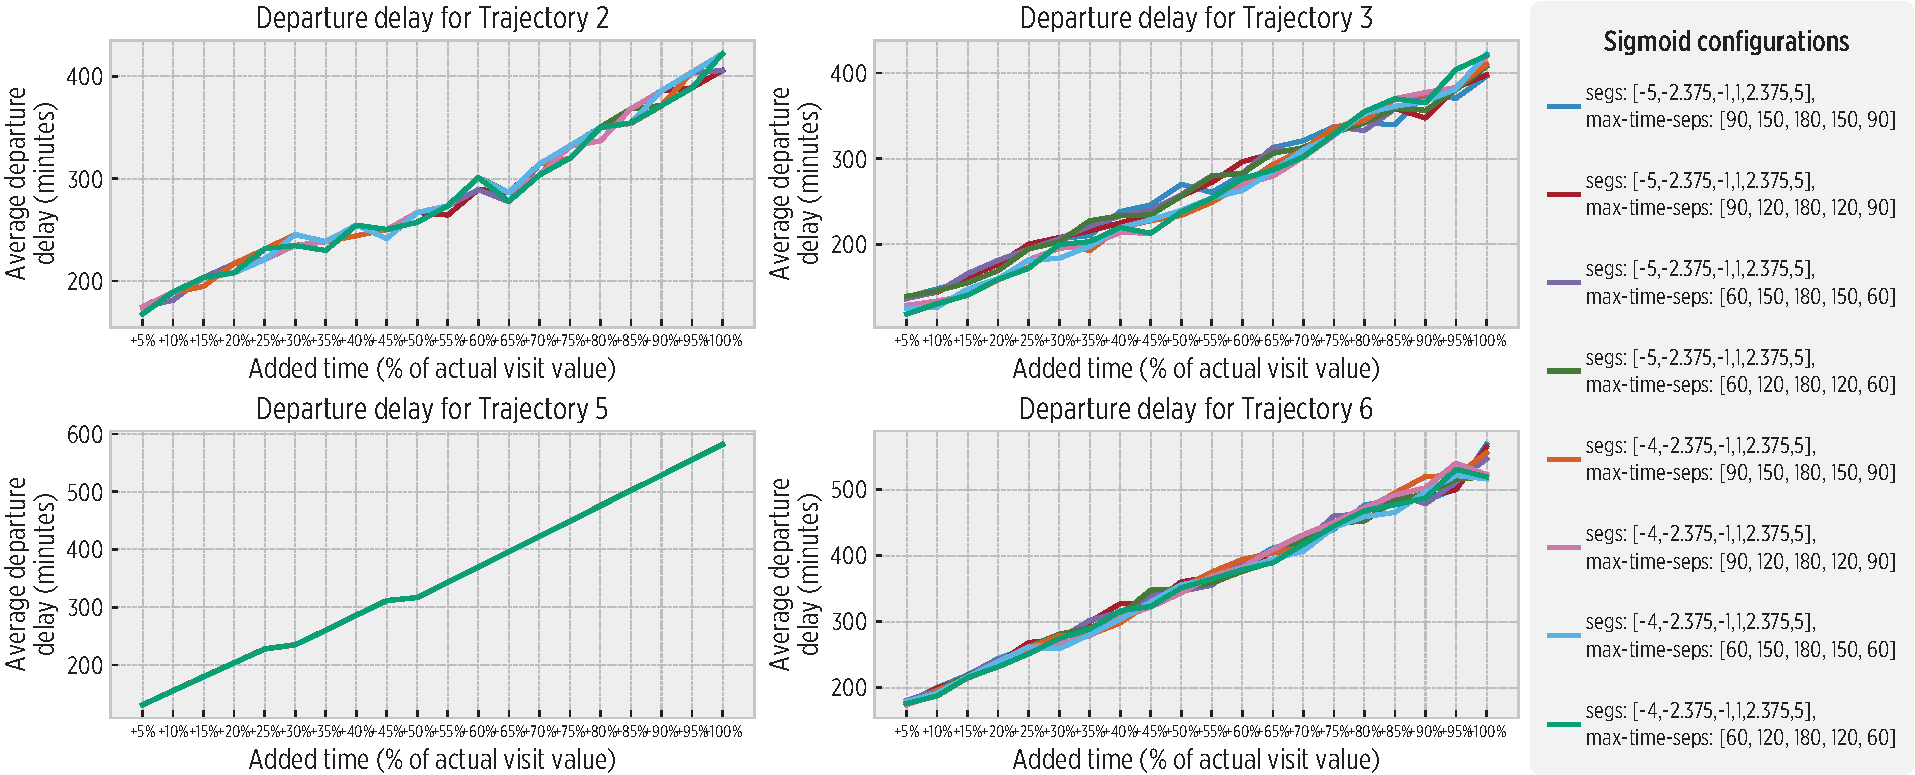
\includegraphics[width=\textwidth]{vectors/experiments/exp-3/exp-3-b-departure-delay-for-slides}
  \makebox[\textwidth][c]{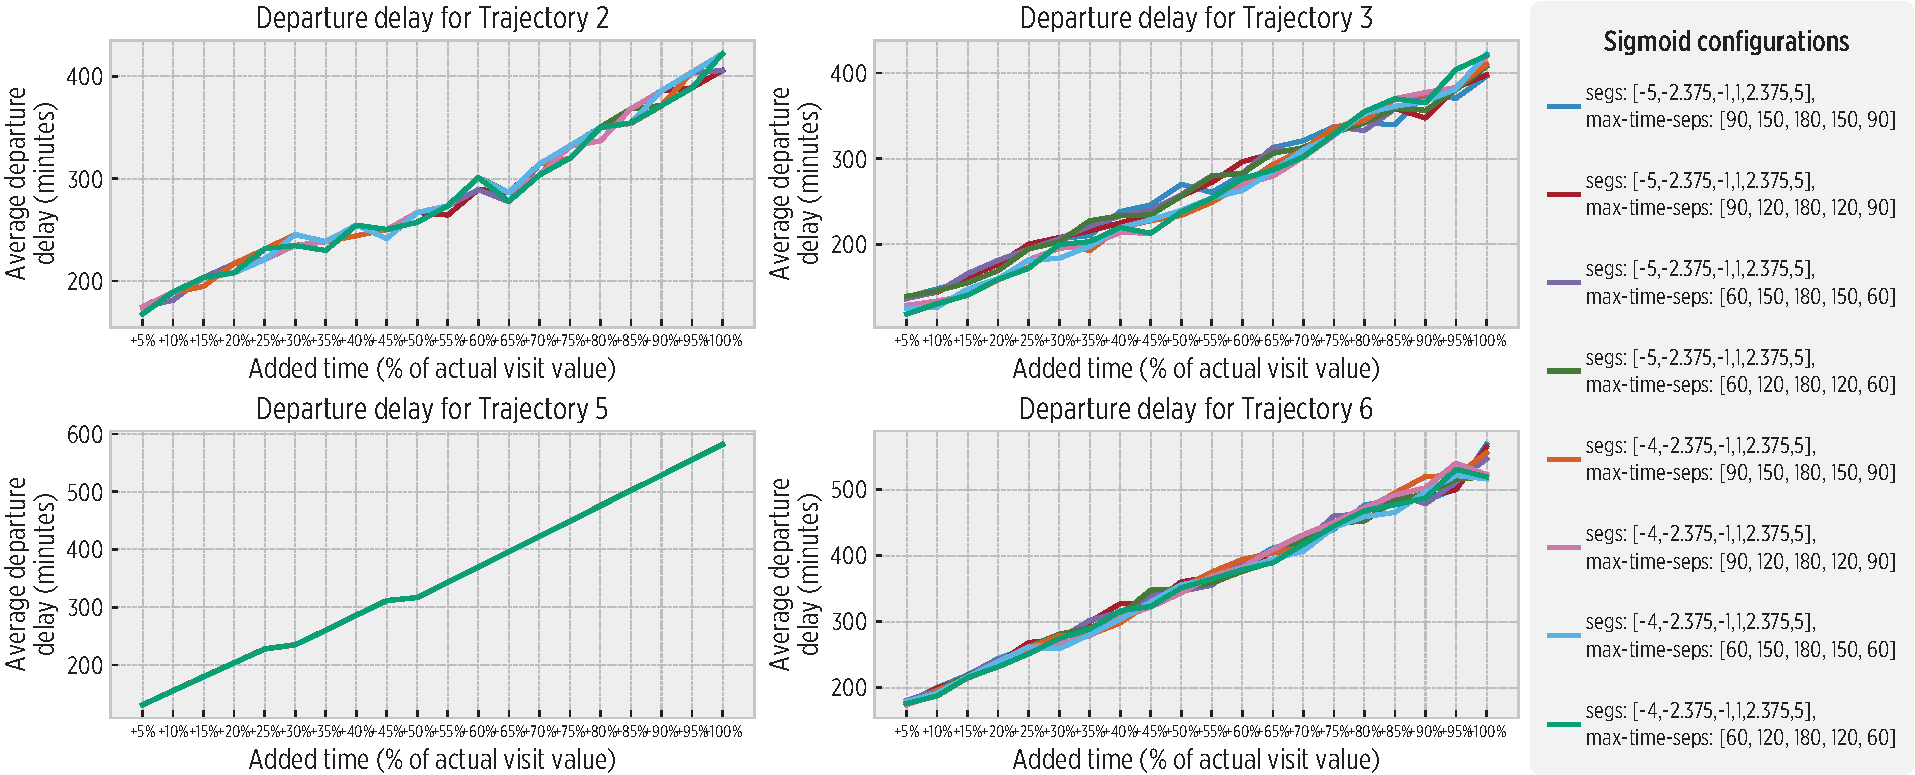
\includegraphics[width=1.05\textwidth]{vectors/experiments/exp-3/exp-3-b-departure-delay-for-slides}}%
  \caption{The evolution of the timespan between the expected and actual departures detected by the system across the different time increments applied to the STM. Similar tendencies are observed, highlighting that the sigmoid sampling allows to identify that user is leaving the stay points before expected.}
  \label{fig:exp-3-departure-delay}
\end{figure}
\end{frame}

\begin{frame}{Preliminary experiments}{Reaction to STM mobility mismatches: Results}
\begin{figure}
  \centering
  %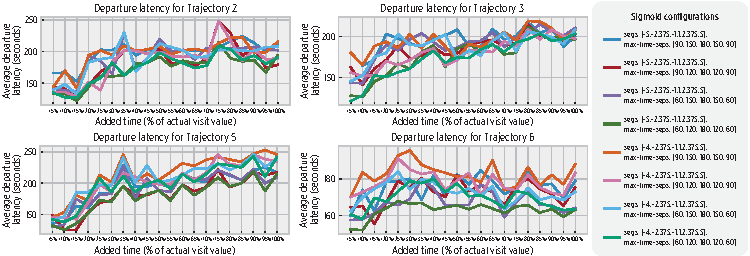
\includegraphics[width=\textwidth]{vectors/experiments/exp-3/exp-3-b-departure-latency-for-slides}
  \makebox[\textwidth][c]{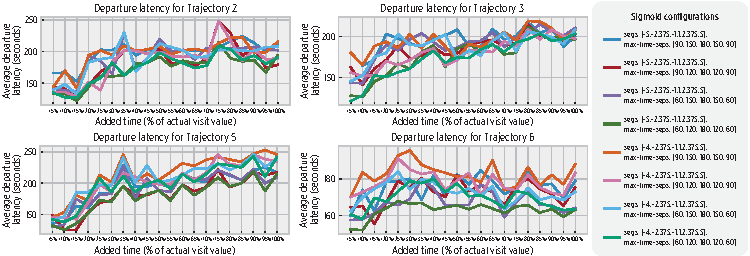
\includegraphics[width=1.05\textwidth]{vectors/experiments/exp-3/exp-3-b-departure-latency-for-slides}}%
  \caption{The variation of the latency values of departures detection when the STM is injured with additional time. The observed values are under the theoretical 360 seconds maximum peak.}
  \label{fig:exp-3-departure-latency}
\end{figure}
\end{frame}

% \subsection{Holistic evaluation}
\begin{frame}{Preliminary experiments}{Holistic evaluation: Description}
\begin{block}{\small \textbf{Description}}
{ 
\small
\begin{itemize}
  \item This experiment was aimed at evaluating the overall spatial-time accuracy performance of the system with all of its component enabled, including:
  \begin{itemize}
    \item The continuous learning of stay points in the STM for adapting GPS sampling rate.
    \item The handling of mobility mismatches.
  \end{itemize}
\end{itemize}
}
\end{block}

\begin{table}
\centering
\renewcommand{\arraystretch}{0.8}
\resizebox{0.8\textwidth}{!}{%
\begin{tabular}{@{}lll@{}}
\toprule

\multirow{3}{*}{\textbf{Geofencing}} & \textbf{Radio distance} ($gf_{distance}$): & $250~m$ \\
 \cmidrule[0.25pt]{2-3}
 & \textbf{Window size} ($gf_{ws}$): & 3 \\

\cmidrule[0.25pt]{1-3}
\multirow{9}{*}{\textbf{Cognitive Controller}} & \multirow{2}{*}{\textbf{Sigmoid segments} ($\Theta_{domain\_segs}$):} & $(-5, -2.375), (-2.375, -1), (-1, 1), (1, 2.375), (2.375, 5)$ \\
 &  & $(-4, -2.375), (-2.375, -1), (-1, 1), (1, 2.375), (2.375, 5)$ \\
\cmidrule[0.25pt]{2-3}
 & \multirow{4}{*}{\textbf{Time separations} ($\Theta_{time\_sep}$):} & $[90, 150, 180, 150, 90]$ seconds \\
 &  & $[90, 120, 180, 120, 90]$ seconds \\
 &  & $[60, 150, 180, 150, 60]$ seconds \\
 &  & $[60, 120, 180, 120, 60]$ seconds \\
 \cmidrule[0.25pt]{2-3}
 & \textbf{On trajectory sampling}: & 30 seconds\\
 \cmidrule[0.25pt]{2-3}
 & \textbf{Conservative sampling}: & 60 seconds\\

\cmidrule[0.25pt]{1-3}
\textbf{Trajectories} & \multicolumn{2}{l}{All ground truth trajectories.} \\

\cmidrule[0.25pt]{1-3}
\textbf{STM} & \multicolumn{2}{l}{Empty}
\\
\bottomrule
\end{tabular}%
}
\caption{Input parameters for the holistic evaluation experiment. The \emph{conservative} sampling refers to the late departure mismatch reaction.}
\label{tab:exp-4-input-parameters}
\end{table}
\end{frame}


\begin{frame}{Preliminary experiments}{Holistic evaluation: Results}
\small 
\vspace{-0.5cm}
{
  \centering
  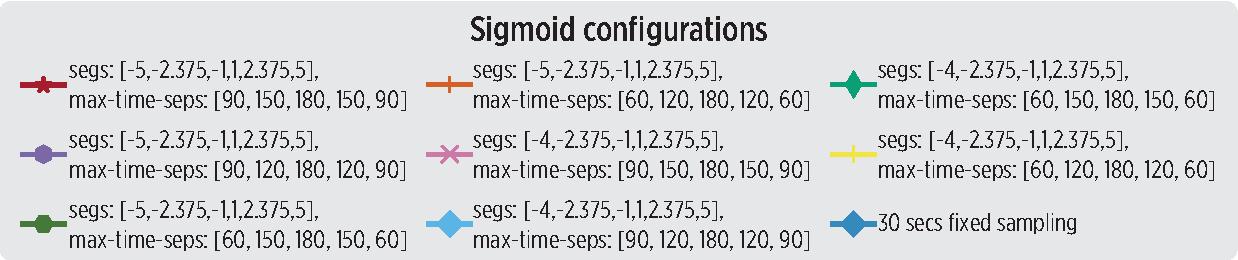
\includegraphics[width=0.7\textwidth]{vectors/experiments/exp-4/exp-4-sigmoid-header-top-row}
  \par 
}

\begin{columns}
\begin{column}[T]{0.48\textwidth}
\begin{block}{\small \textbf{Arrival latency}}
{
  \centering
  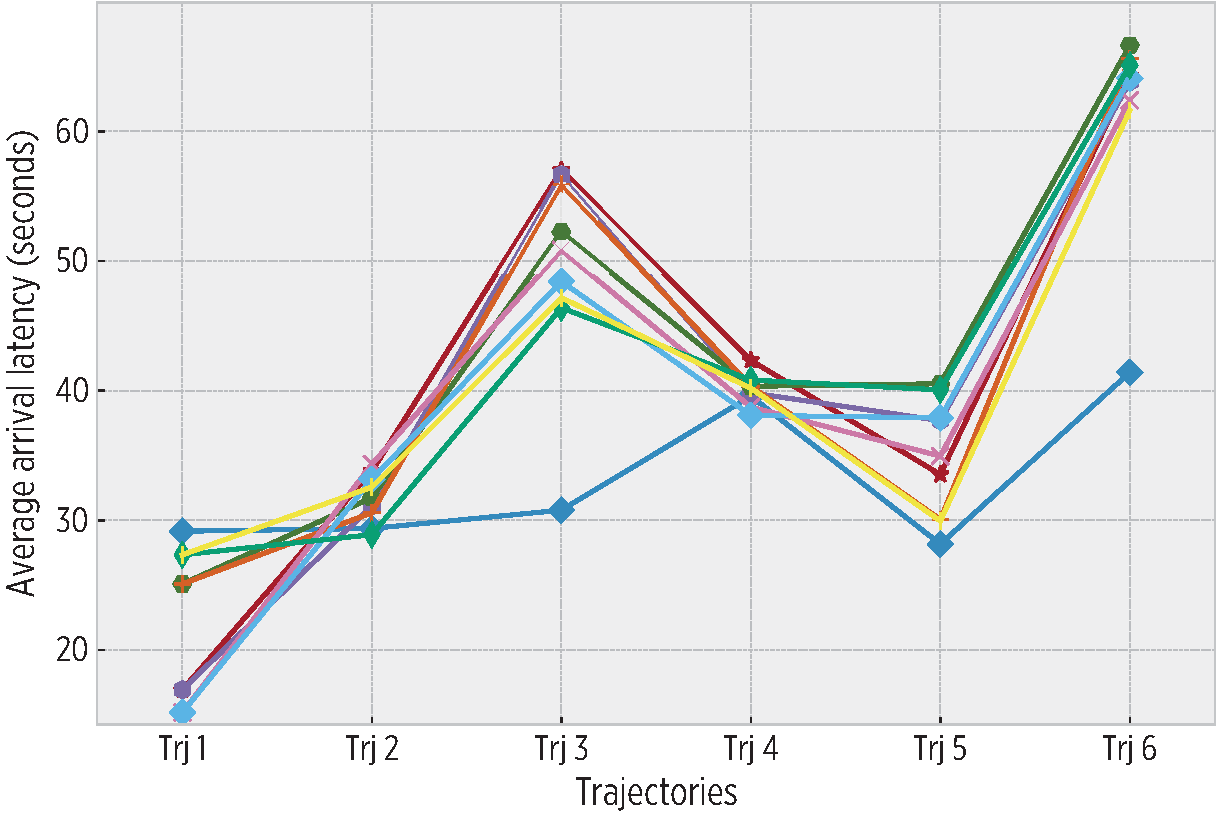
\includegraphics[width=\textwidth]{vectors/experiments/exp-4/exp-4-arrival-latency-for-slides-v2}
  \captionof{figure}{Arrival latency observed by the platform in experimental trials. The largest average value is below 65 seconds, explained by the fact that 2 location updates must be collected by the \emph{Geofencing} module before identifying an arrival event.}
  \par 
}
\end{block}
\end{column}

\begin{column}[T]{0.52\textwidth}
\begin{block}{\small \textbf{Departure latency}}
{
  \centering
  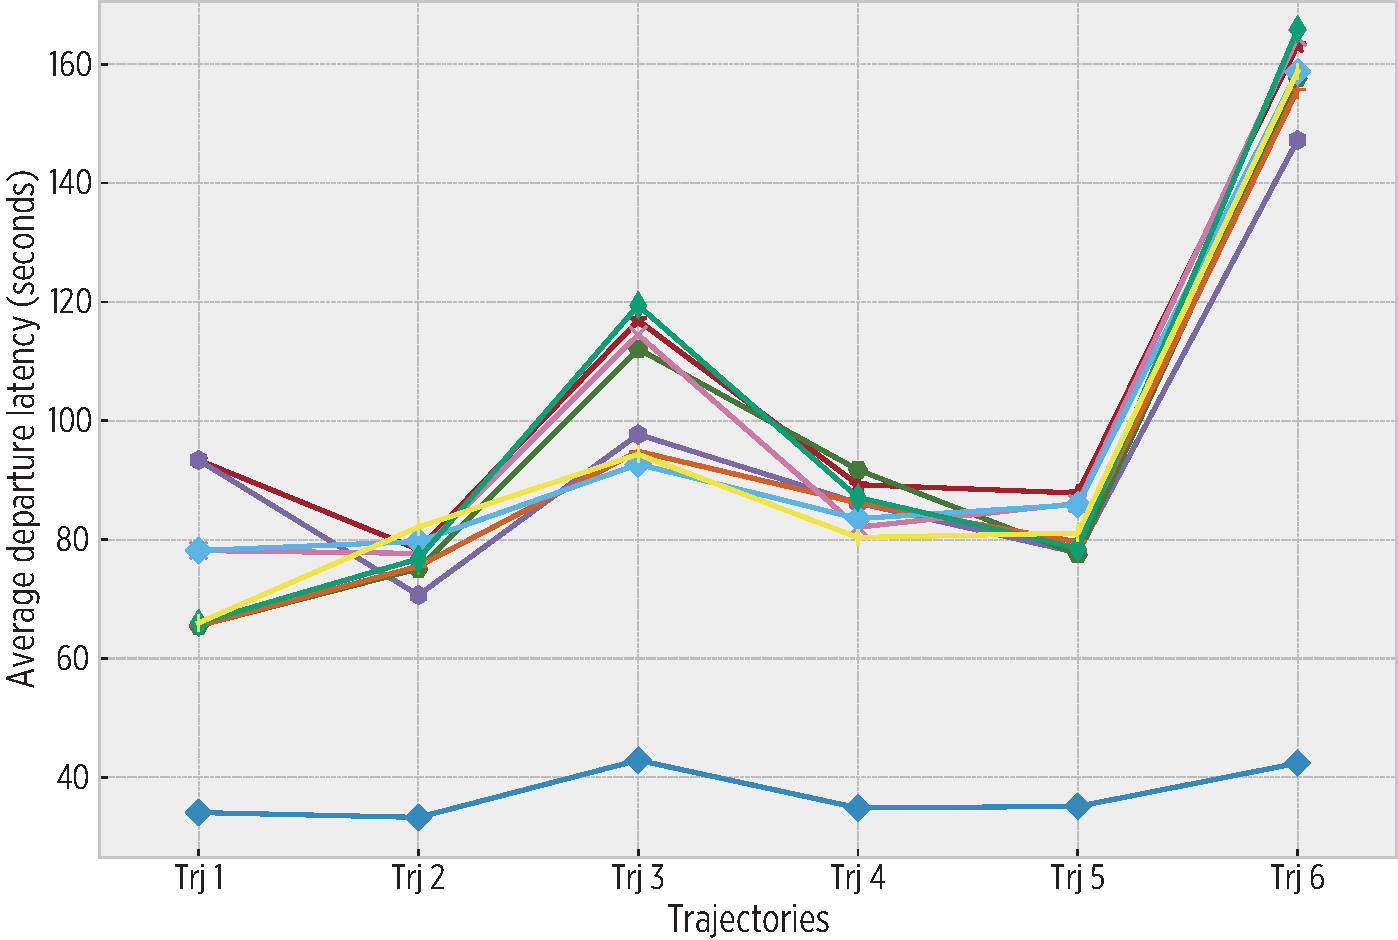
\includegraphics[width=\textwidth]{vectors/experiments/exp-4/exp-4-departure-latency-for-slides-v2}
  \captionof{figure}{Departure latency observed by the platform across performed experimental trials. The latencies are within 65 and 165 seconds, which is aligned with the different values specified to the CC for its sigmoid-driven sampling.}
  \par
}
\end{block}
\end{column}
\end{columns}

\end{frame}


\begin{frame}{Preliminary experiments}{Holistic evaluation: Results}
\small 
\vspace{-0.5cm}
{
  \centering
  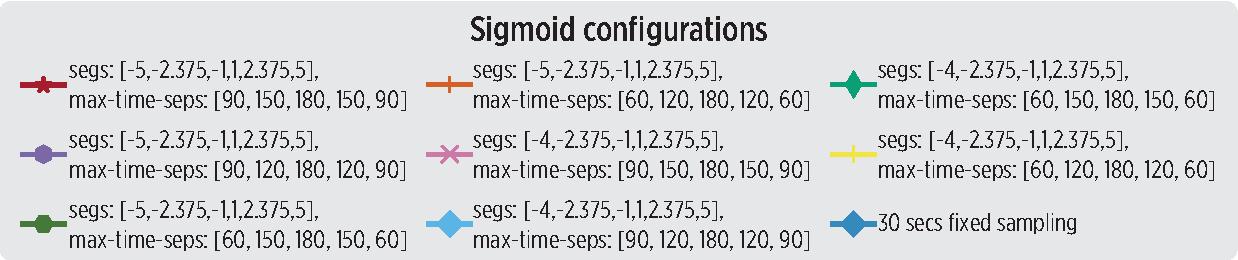
\includegraphics[width=0.7\textwidth]{vectors/experiments/exp-4/exp-4-sigmoid-header-top-row}
  \par 
}


\begin{columns}
\begin{column}[T]{0.5\textwidth}

\begin{block}{\small \textbf{Arrival distance difference}}
{
  \centering
  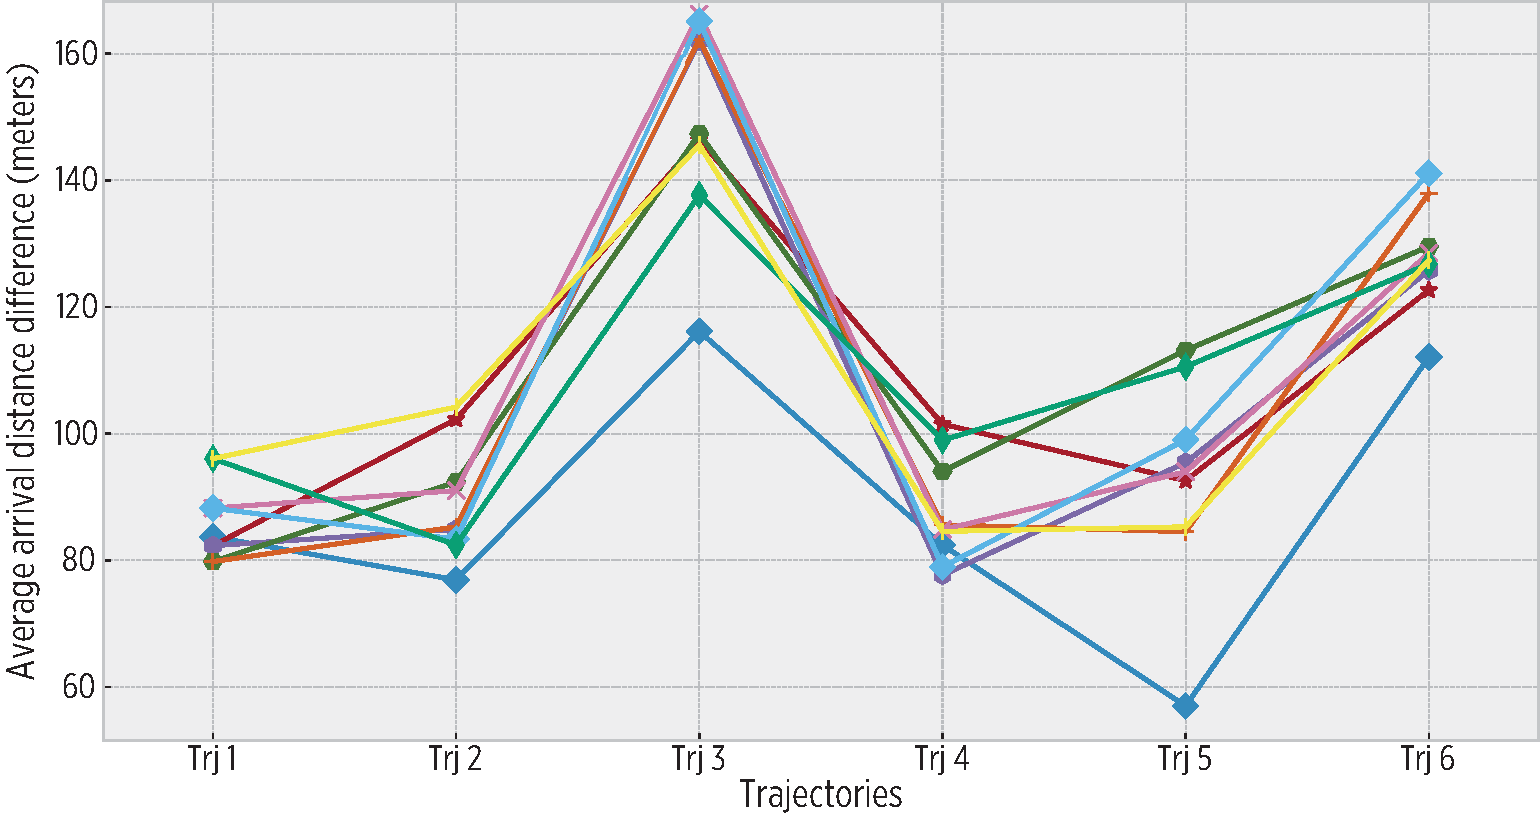
\includegraphics[width=\textwidth]{vectors/experiments/exp-4/exp-4-arrival-distance-for-slides-v2}
  \captionof{figure}{Arrival distance difference detected by the system throughout the different experimental trials. The values are shorter than for departure distance due to the decreasing speed that user describes when arriving to a stay point.}
  \par
}
\end{block}
\end{column}

\begin{column}[T]{0.5\textwidth}
\begin{block}{\small \textbf{Departure distance difference}}
{
  \centering
  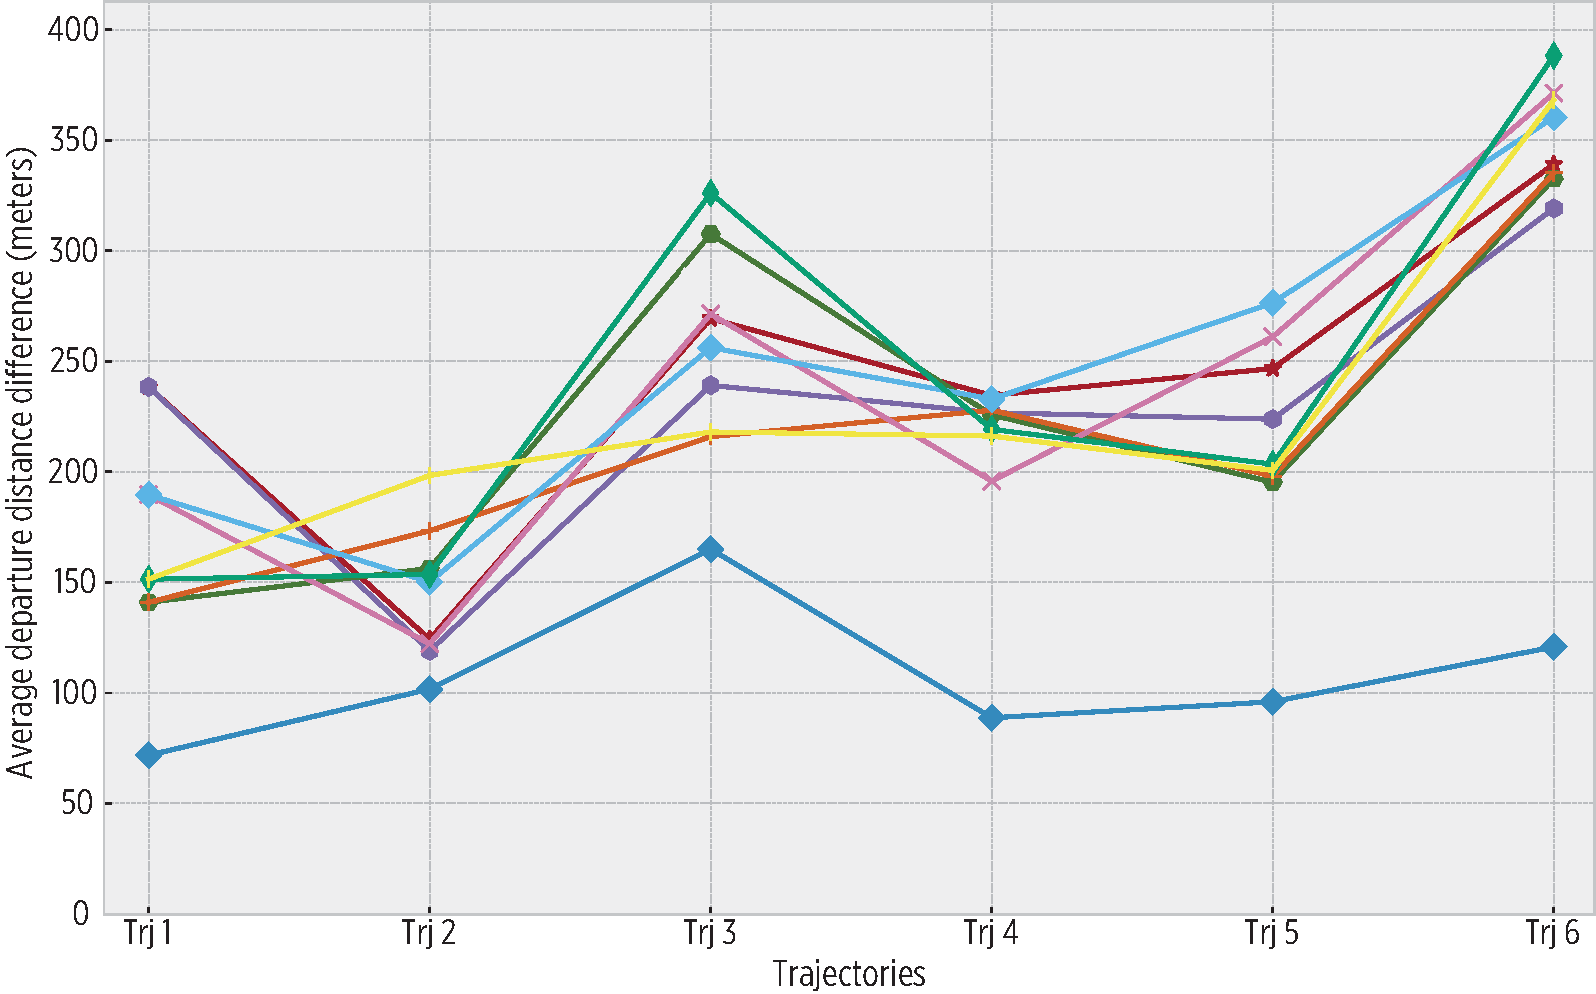
\includegraphics[width=\textwidth]{vectors/experiments/exp-4/exp-4-departure-distance-for-slides-v2}
  \captionof{figure}{Departure distance difference detected by the system throughout the different experimental trials. The larger distance differences are caused by the high speed with which user leaves the stay points (mostly using a vehicle as transportation mode).}
  \par
}
\end{block}

\end{column}
\end{columns}

\end{frame}



\begin{frame}{Preliminary experiments}{Holistic evaluation: Results}
\small
\vspace{-0.5cm}
{
  \centering
  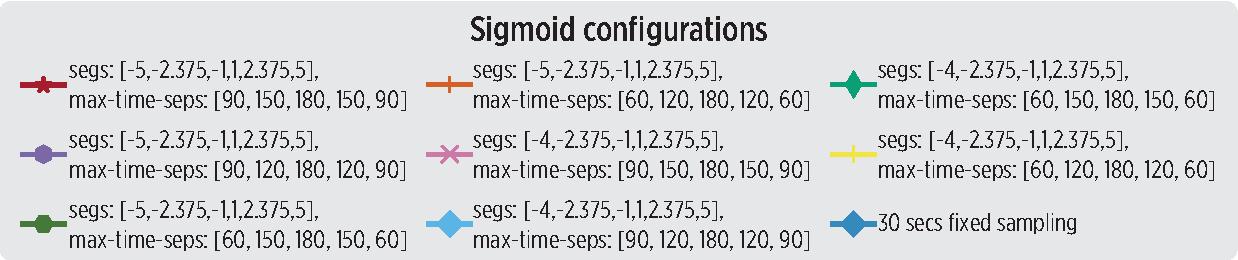
\includegraphics[width=0.7\textwidth]{vectors/experiments/exp-4/exp-4-sigmoid-header-top-row}
  \par 
}

\begin{columns}
\begin{column}[T]{0.5\textwidth}

\begin{block}{\small \textbf{Trajectory distance difference}}
{
  \centering
  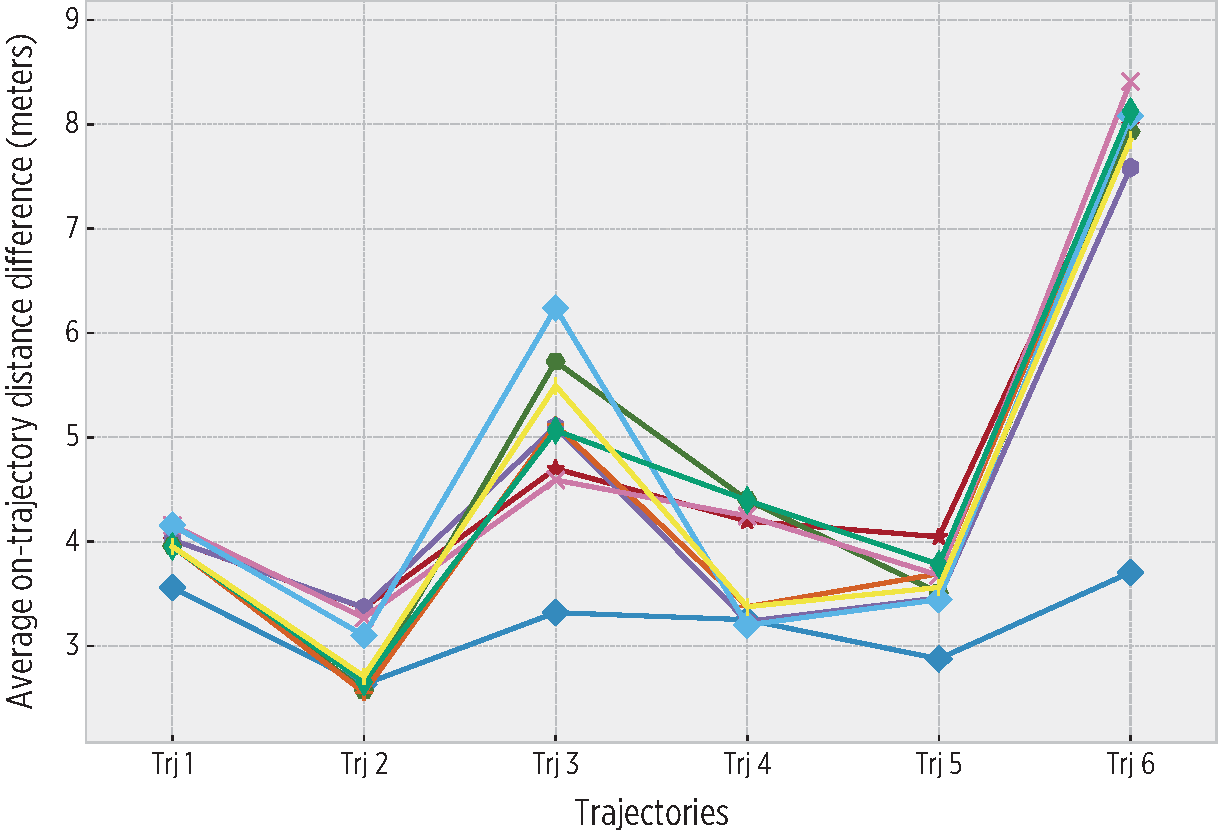
\includegraphics[width=\textwidth]{vectors/experiments/exp-4/exp-4-on-trajectory-distance-for-slides-v2}
  \captionof{figure}{The average distance of equivalent trajectory segments during experimental trials. The values are enclosed within $2.5~m$ and $8.5~m$, with the 30 seconds sampling obtaining the lowest values in each trial.}
  \par
}
\end{block}

\end{column}

\begin{column}[T]{0.5\textwidth}
\begin{block}{\small \textbf{Overall reduction of location update requests}}
{
  \centering
  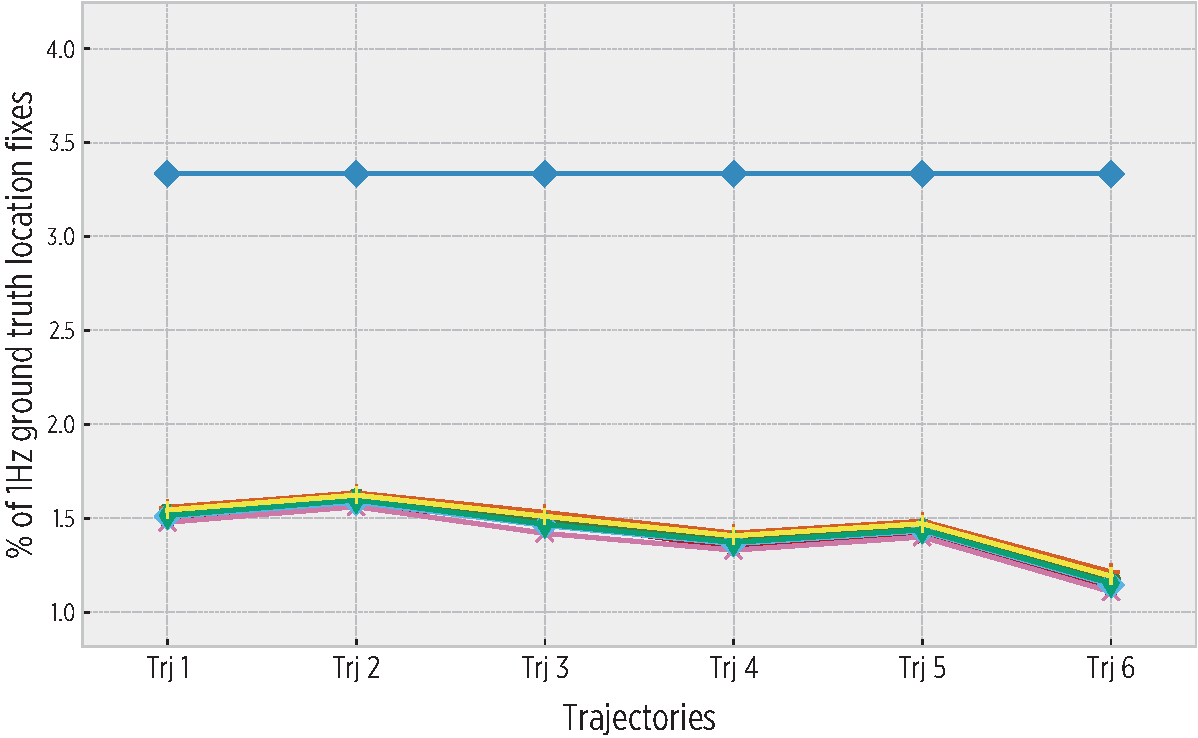
\includegraphics[width=\textwidth]{vectors/experiments/exp-4/exp-4-location-requests-for-slides-v2}
  \captionof{figure}{The proportion of location update requests employed by each experimental trial with respect to the corresponding $1~Hz$ ground truth trajectory. All of the parameter combinations outperform the 30 seconds sampling period, which provides a rough estimation of the energy savings that the system could achieve in on-device implementations.}
  \par
}
\end{block}
\end{column}
\end{columns}
\end{frame}

% \subsection{Feasibility of on-device stay points detection}
\begin{frame}{Preliminary experiments}{Energy saving expectations of on-device stay points detection}
\small
% \vspace{-0.5cm}
\begin{columns}
\begin{column}{0.55\textwidth}
\begin{block}{\small \textbf{Description}}
\begin{itemize}
  \item This experiment explored whether a smartphone could detect stay points by itself, and the energy savings of such implementation with respect of typical Mobile Cloud Computing (MCC) based solutions.
  % \item Typical solutions implement a Mobile Cloud Computing (MCC) approach on which the smartphone only collects and offloads the processing to external servers.
\end{itemize}
\end{block}
\end{column}

\begin{column}{0.4\textwidth}
\begin{table}
\centering
\renewcommand{\arraystretch}{0.8}
\resizebox{0.95\textwidth}{!}{%
\begin{tabular}{lll}
\toprule
\multirow{2}{*}{\textbf{Stay Points Detector}} & \textbf{Time threshold} ($\delta_{time}$): & $45~min$ \\
\cmidrule[0.25pt]{2-3}
 & \textbf{Distance threshold} ($\delta_{distance}$): & $500~m$ \\

\cmidrule[0.25pt]{1-3}
\textbf{Sampling periods}: & \multicolumn{2}{l}{30, 60, 90, 120, 150 seconds} \\
\bottomrule
\end{tabular}
}
\caption{Input parameters for the energy saving expectations of on-device stay points detection experiment.}
\label{tab:exp-energy-performance-input-parameters}
\end{table}
\end{column}
\end{columns}

\begin{figure}
  \centering
  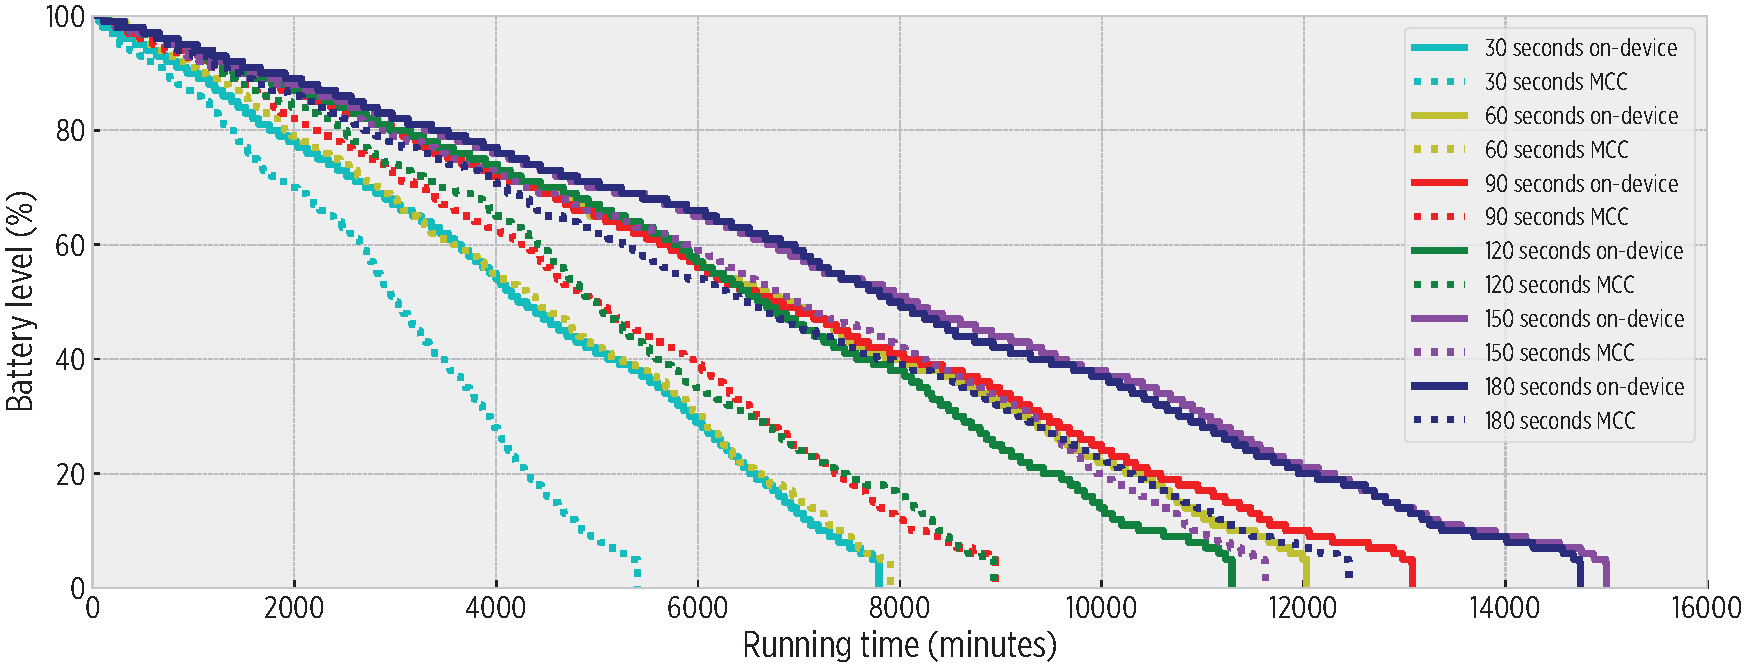
\includegraphics[width=\columnwidth]{vectors/local-poi-article/plot-energy-performance-r2-for-slides}
  \caption{Energy performance comparison of on-device vs. MCC sample apps using different GPS sampling periods. Each of the on-device trials last longer than its corresponding remote implementation.}
\end{figure}

\end{frame}

% \begin{frame}{Preliminary experiments}{Energy saving expectations of on-device stay points detection: Results}
% \small
% \begin{figure}
%   \centering
%   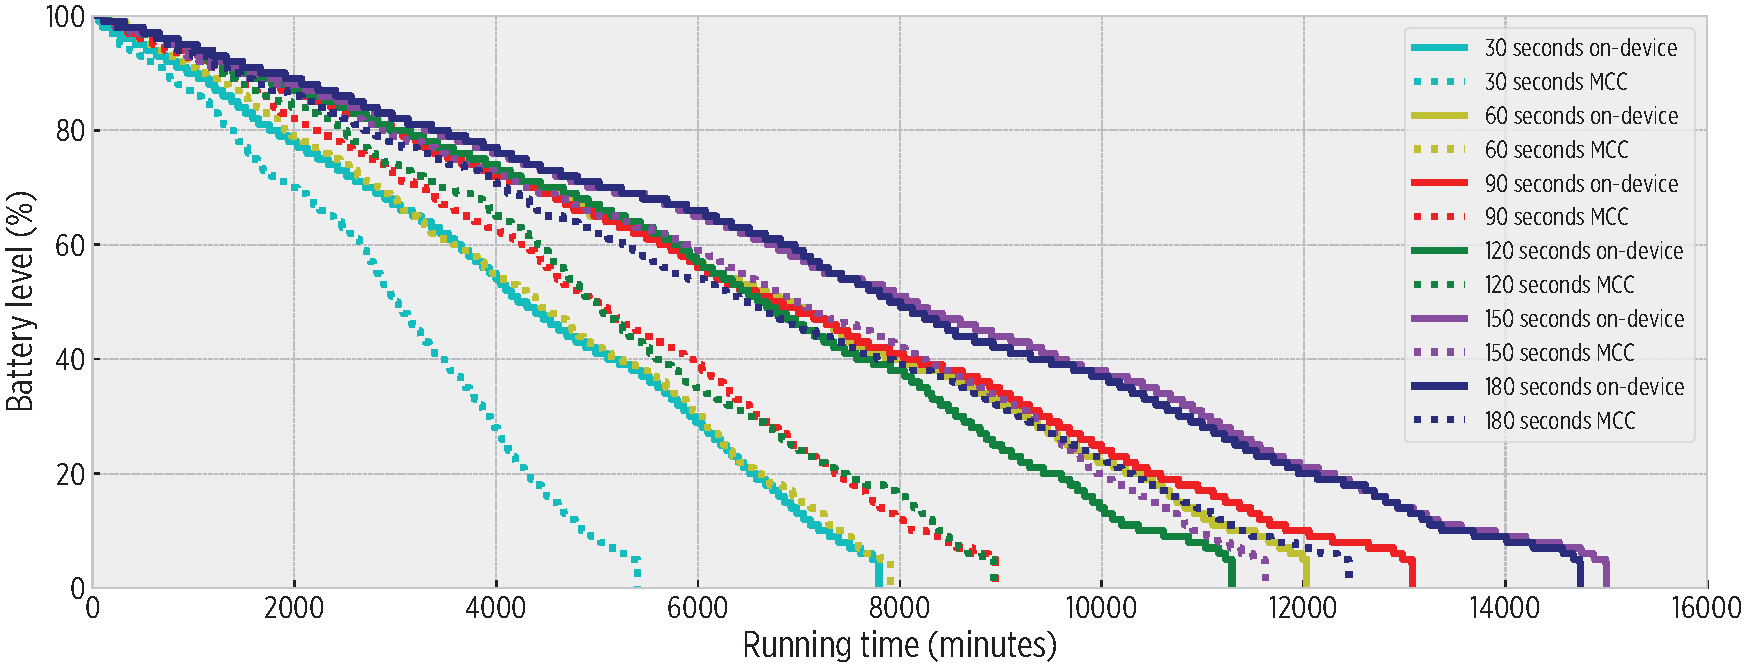
\includegraphics[width=\columnwidth]{vectors/local-poi-article/plot-energy-performance-r2-for-slides}
%   \caption{Energy performance comparison of on-device vs. MCC sample apps using different GPS sampling periods. Each of the on-device trials last longer than its corresponding remote implementation.}
%   \label{fig:energy-performance-on-device-mcc-comparison}
% \end{figure}
% \end{frame}

% \subsection{Energy consumption of fixed-sampling periods}
\begin{frame}{Preliminary experiments}{Energy consumption of fixed-sampling periods: Description}
\small
\begin{block}{\small \textbf{Description}}
\begin{itemize}
  \item This experiment evaluated the impact of sampling adaptations based on fixed sampling rates on the energy consumed by the proposed CDS.
  \item All system components were enabled, with the exception of the sigmoid sampling of the CC.
  \item The CC followed fixed sampling periods depending on the current mobility state recognized by the system.
  \item The experiment also demonstrated the mobility awareness that the system provides to the smartphone (STM).
\end{itemize}
\end{block}


\begin{table}
\centering
\renewcommand{\arraystretch}{0.8}
\resizebox{0.8\textwidth}{!}{%
\begin{tabular}{@{}lll@{}}
\toprule
\multirow{2}{*}{\textbf{Stay Points Detector}} & \textbf{Time threshold} ($\delta_{time}$): & $45~min$ \\
\cmidrule[0.25pt]{2-3}
 & \textbf{Distance threshold} ($\delta_{distance}$): & $500~m$ \\

\cmidrule[0.25pt]{1-3}
\multirow{3}{*}{\textbf{Geofencing}} & \textbf{Radio distance} ($gf_{distance}$): & $250~m$ \\
% \cmidrule[0.25pt]{2-3}
% & \textbf{Pivot parameter} ($gf_{pv}$): & center \\
 \cmidrule[0.25pt]{2-3}
 & \textbf{Window size} ($gf_{ws}$): & 3 \\

\cmidrule[0.25pt]{1-3}
\multirow{2}{*}{\textbf{HAR module}} & \textbf{Individual window length}: & $5$ seconds \\
\cmidrule[0.25pt]{2-3}
 & \textbf{Meta-window size} ($HAR_{mws}$): & $5$ \\

\cmidrule[0.25pt]{1-3}
\multirow{4}{*}{\textbf{Cognitive Controller}} & \multirow{2}{*}{\textbf{Smartphone 1}:} & On trajectory sampling periods: 30 seconds\\
 &  & On stay point sampling period: 30 seconds \\
\cmidrule[0.25pt]{2-3}
 & \multirow{2}{*}{\textbf{Smartphone 2}:} & On trajectory sampling period: 30 seconds\\
 &  & \begin{tabular}[c]{@{}l@{}}On stay point sampling period:\\one in the set $\{ 60, 90, 120, 150, 180 \}$ seconds\end{tabular} \\

\bottomrule
\end{tabular}%
}
\caption{Input parameters for the energy consumption of fixed-sampling periods experiment.}
\label{tab:exp-6-input-parameters}
\end{table}
\end{frame}

\begin{frame}{Preliminary experiments}{Energy consumption of fixed-sampling periods: Results}
\vspace{-0.4cm}
{
  \centering
  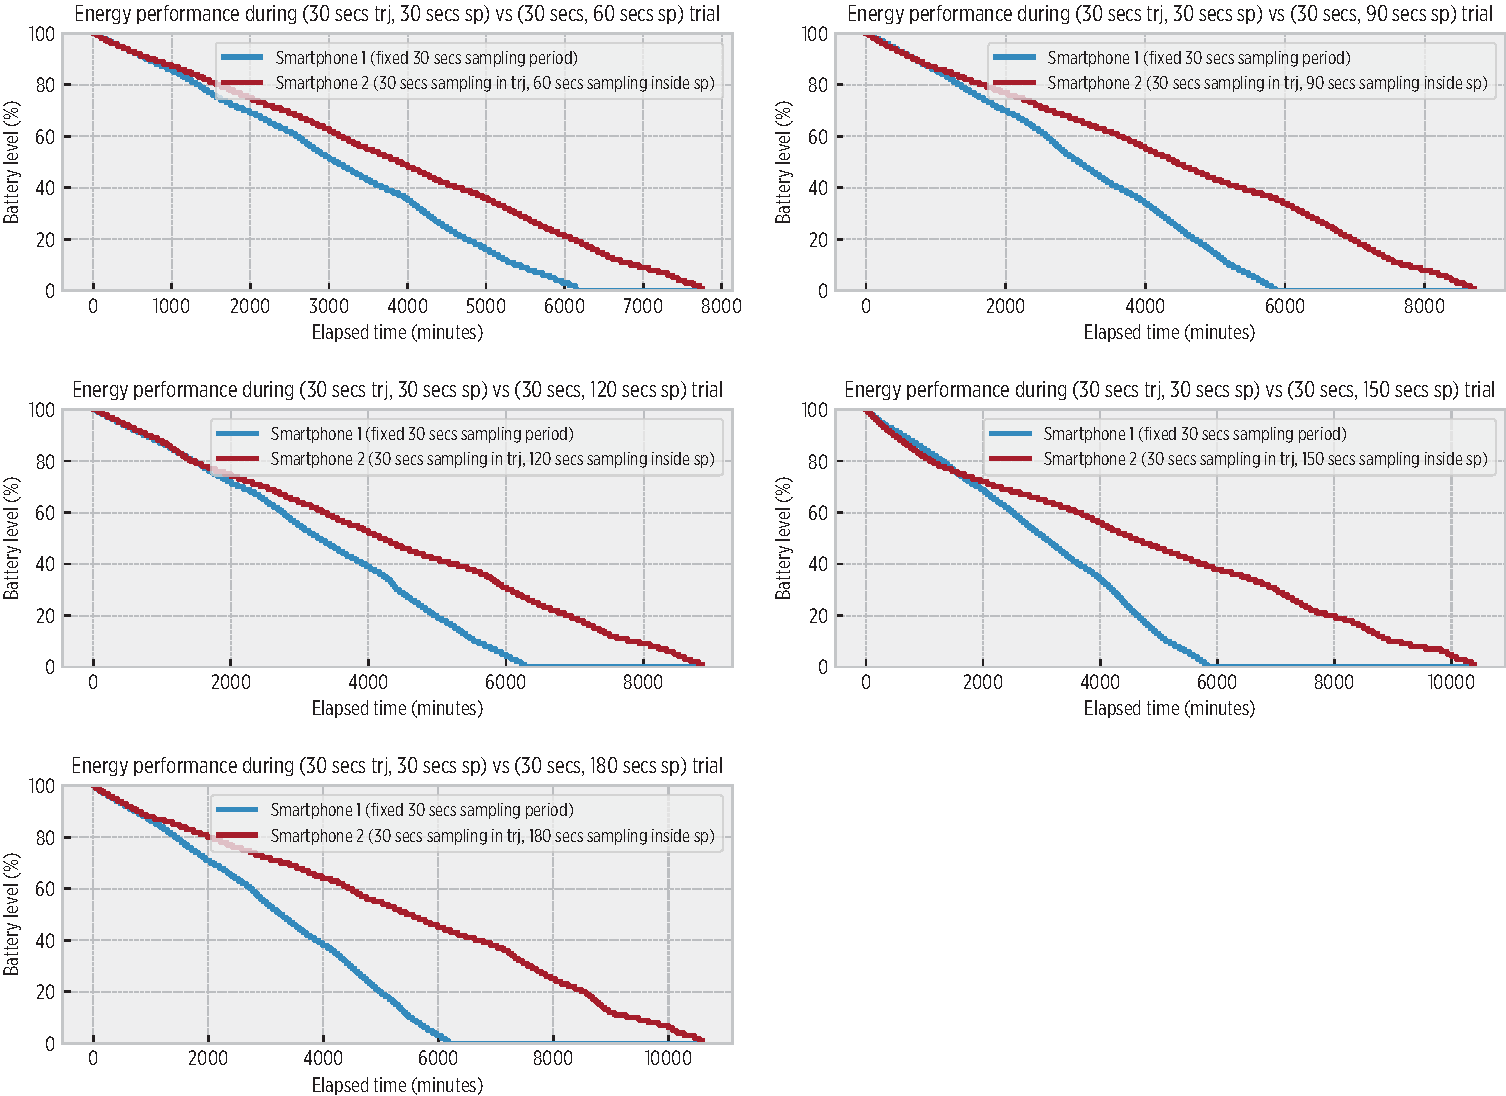
\includegraphics[width=0.85\textwidth]{vectors/experiments/exp-6/exp-6-energy-burnout}
  \captionof{figure}{Energy performance of a fixed 30 seconds sampling versus a basic sampling adaptation consisting in a 30 seconds sampling in trajectory mode and a slower sampling rate during stay point mode. The separation between the lines in each plot starts after the system learns the stay points with the largest weight in user mobility (home and work places).}
  \par
}
\end{frame}

\begin{frame}{Preliminary experiments}{Energy consumption of fixed-sampling periods: Results}
\begin{figure}
  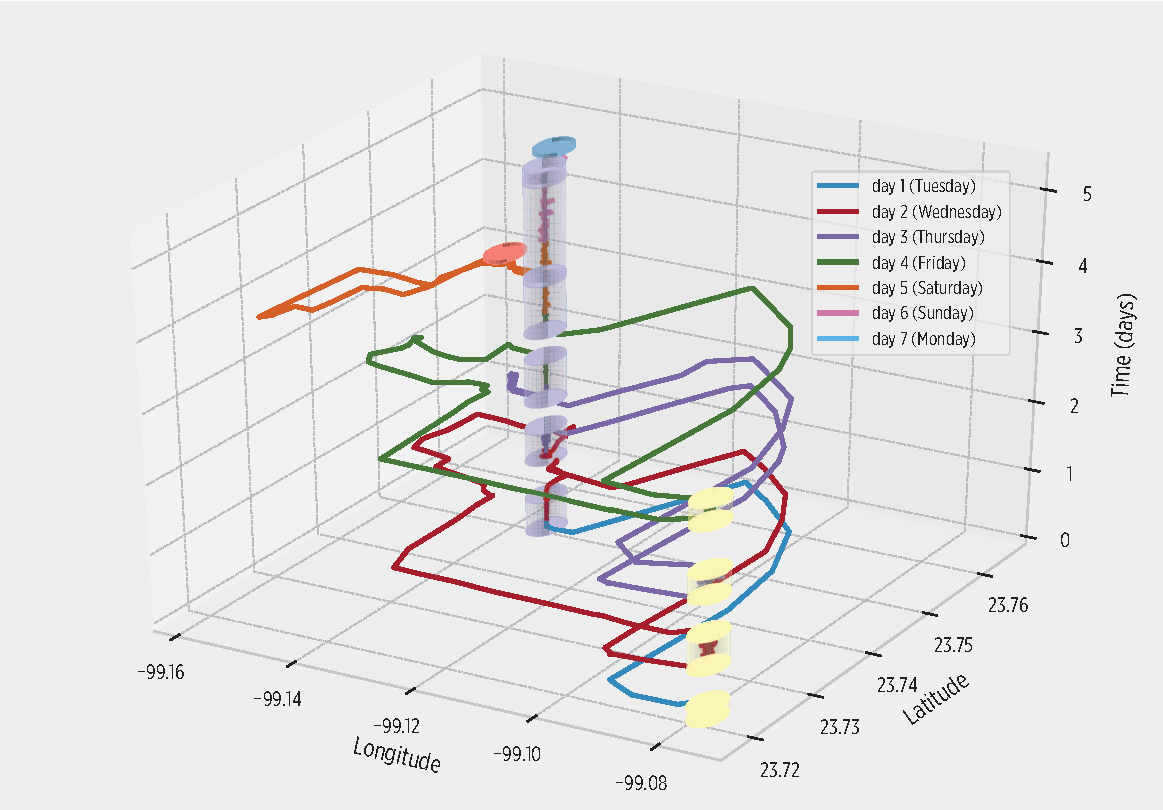
\includegraphics[width=0.8\textwidth]{vectors/experiments/exp-6/exp-6-map-trj-4-adaptive-sampling-60-sp}
  \caption{The information autonomously learned by the STM during the trial corresponding to the 30 seconds in trajectory and 60 seconds in stay point sampling scheme. The height of cylinders corresponds with the stay time during each stay point visit.}
  \label{fig:exp-6-stm-60-seconds-sp}
\end{figure}
\end{frame}

\begin{frame}{Preliminary experiments}{Comparison with other solutions}
\begin{table}[]
\centering
\small
\renewcommand{\arraystretch}{1.2}
\begin{tabular}{@{}p{1cm}p{1.8cm}p{1.6cm}p{1.4cm}p{1cm}p{1cm}@{}}
\toprule
\textbf{Work} &
\textbf{Purpose} &
\textbf{Mobility type} &
\textbf{Involved sensors} &
\textbf{Trajectory tracking} &
\textbf{Place learning} \\ 
\midrule

\textbf{SenseLess} &
Location tracking &
Walking, static &
Accelerometer, GPS &
Yes &
No \\

\cmidrule[0.25pt]{1-6}
\textbf{SmartDC} &
Place tracking &
Not specified &
Cellular id, Wi-Fi, GPS&
No &
Yes \\

\cmidrule[0.25pt]{1-6}
Proposed system &
Location and place tracking &
Static, walking, biking, vehicle &
Accelerometer, GPS &
Yes &
Yes \\

\bottomrule
\end{tabular}%

\caption{Features comparison of proposed system and representative existing solutions.}
\end{table}
\end{frame}
